\section{Electron beam lithography}

\subsection{Misc}
- never close the 'Smart SEM' window\\
- never close the 'gun monitor'\\
- if the 'Raith150-two' window is closed, use the following passwords when you open it: login: unsw, pass: unsw\\
- Working Distance (WD): distance between the sample and the source of electrons. \\
- XYZ coordinate:\\
coordinate of sample inside the raith. XY: horizontal coordinates. $0.1<Z<22.7$. Z never equals zero. Origin: middle of sample holder. \\
- UVW Global:\\
Coordinate for an existing geometry.\\
- UVW Local:\\
Coordinate of a pattern inside an existing geometry. The origin of the UVW Local coordinate is on a point which does not belong to the geometry you want to create (like crosses on corner of chip). This prevent the microscope to expose with electrons the area where your future pattern will be.\\
- InLens (viewing method): 0 to 20\,kV\\
- SE2 (viewing method): 20 to 30\,kV\\
- imaging: internal mode ; writing: external mode\\
- always \boxed{read} before \boxed{adjust} to coordinates!!\\
- demo pattern in \textit{users/sylvain/GDSII/demo} \\
- Good brightness settings for 30um aperture: 50.5 ; Good contrast settings: 29.2\\
- Good brightness settings for 20um aperture: 49.4 ; Good contrast settings: 32.9\\
 
\subsection{Important}

- Expose the chip as less as possible in internal (viewing) mode\\

\subsection{Imaging}

focus and stigmatize on the feature\\

To prevent damage (if they are possible) use a  low exposure, like 2\,kV.\\

in the `scanning' tab:\\
- choose a scan speed\\
- ensure that `freeze on = end of frame'\\
- record picture\\


\subsection{Designs EBL patterns}

keep some mesa away from your EBL geometry to put gold drops on it, and to focus and stigmatize without exposing the area where your pattern will be\\
Ideally, your gold balls and contamination dot should be not more than 300\,$\mu$m away from your write field.\\

the first alignment marks are done at the same time as the ohmic layer\\

add alignment marks with the EBL in order to do accurate alignment (if necessary, this will add one more step in the nanofab process)\\
! 4 alignement crosses in one write field !\\

fines gates and auto alignement marks should be at the middle of a write field.\\

in the Raith software:\\
- \boxed{create~structure} to create a pattern\\
- drag the structure name in your mail structure\\


\subsection{Prologue}

Using the EBL, get the coordinates of 3 points around each device to use for 3 points alignment purpose.\\

\textbf{** PMMA spinning **}\\

\subsubsection{Aim}
to know the thickness of resist to spin\\

What is the thickness of metal needed: 50\,\AA~Ti and 150\,\AA~Au = 200\,\AA \\

Wanted thickness of PMMA: 400\,\AA  ~at least.\\
(1.5 to 2 $\times$ thickness of metal (better to use a factor 2))\\


Spin PMMA 3 on chip (check thickness):\\
- dispense resist at 500 rpm for 5\,s.\\
- spin at 6000 rpm for 30\,s.\\
- bake at 180$^{\circ}$C for 90\,s\\


\textbf{** deposit gold spheres **}\\

\subsubsection{Aim}
deposit gold sphere to focus the electron beam (later)\\

put your chip under microscope\\

focus on the surface of the chip. Choose a corner to focus on, it is easier.\\

using the paper clip, put some liquid containing gold balls:\\
plce the edge of a drop between 2 ohmics at the extremity of a row of ohmics (extremely tricky).\\

write the location of the edge of your drop on your drawing\\

wait for the liquid to dry (dry when it forms a kind of dirty black circle)\\

Take your chip to the EBL.\\

\newpage


\subsection{Recipe}

On the left hand side of the Raith, open the square door and take the Universal Sample Holder (USH).\\

clamp your sample in the Universal Sample Holder (prefer left holders).\\

put the USH back in the Raith, \underline{ensure is it clamped properly}\\

click on \boxed{load~sample} to load the sample. This starts a procedure to bring the sample from the load lock to the electrons source, via opening/closing valves\\

When the loading is finish, move the sample upwards to a position of about 20-21 mm (WD from 8 to 10mm). 20.5\,mm is usually preferred.\\

Open the wafer file "USH 150mm" (or something similar) in File/open waferfiles.\\

Hold \boxed{ctrl} + click on right mouse button to bring the pink square (location of the electrons beam) on the chip (on screen).\\
Wait for the sample to stop moving.\\

Turn the EHT on \\

check voltage. 10\,kV is standard (usually 10-20\,kV is used)\\

Check aperture \\
To change the EHT settings, go in the tab `gun', and double click on the EHT window. Aperture: circle through which electrons goes.\\
Use 30$\mu$m to image\\
Use 20$\mu$m to write\\

Viewing methods: InLens prefered compare to SE2.\\
InLens has a boost mode to boost the electron beam voltage to +8kV, but the maximum voltave is 30\,kV. So never goes above 22\,kV. \\

\subsubsection{Step 1: Specify UVW coordinates}
you need to be accurate if you want to use the markers coordinate to find them. Note witch corners you are using as an origin. A magnification of $\approx$500$\times$  is enough to setup the global coordinate system.\\

Set up a low magnification (button on top menu)\\

Using the viewing mode, and open the blanker ($\approx$ shutter) by clicking on \boxed{beam~on/off}\\

Zoom and focus on the left right corner. Sketch which feature of the corner you are using as an origin.\\

plot the cross or target (\boxed{green~target?}), and position the corner at the center of the cross\\

in the UVW global menu, click on \boxed{adjust} to set the origin at the current point (corner)\\

\boxed{read} the coordinates for this first point\\

to set up a second coordinate point, focus on the right corner and click \boxed{read} on the \textit{label 2} line.\\

\boxed{adjust} the coordinates for this second point\\

if the "calculated angle" is in red, click adjust again to rotate the sample\\

If some vibrations occurs, adjust the focus wobble\\


\subsubsection{Step 2: Focus the electron beam (set the Working Distance)}

 start with a low magnification\\

find the gold drop using U,V coordinates.
zoom on the gold balls\\

while zooming, focus on the gold balls\\
It is easier to focus on an area with a lot of balls. Just be carefull to chose a flat layer of balls to focus on\\

zoom (small inset) on a few balls, once the focus is good (round shape), stigmatize to have sharper edges.\\

Good focus and stigmatization = spheric gold balls with sharp edges.\\

close the blanker\\

go back to a low magnification ($\approx 1000 \times$)\\

\textbf{Remove the stigmatization mode !!}\\


\subsubsection{Step 3: Move to your first mark and measure the current}
measure your current before 3 points alignement cause it create some offset (negliglble in theory, but...)\\

Move to your 1rst mark using its coordinate. Check you can see it.\\

hit \boxed{beam~current}\\

choose "faraday cup on holder", check "drive back" is on\\

hit \boxed{measure}\\



\subsubsection{Step 4: 3 points alignment (setup the local coordinates)}

if the 3 points alignment is needed, set-up the global coordinates system accurately.\\

load your design, rotate it to match the one you want to write (according to locatio of the mesa and orientation of the ohmics).\\

Get the local coordinates of your 3 points alignment marks from your design by double-clicking on it.\\

check that your magnification allows you to cover just the size of your marker (to not expose the resist around your marker): 1\,k$\times$ is preferred.\\

load your geometry, and write the coordinates of your 3 points\\

! be careful when you switch between mm and $\mu$m !\\

Setup point 1:\\
- enter U,V coordinates (obtain by scanning) of your 1$^{rst}$ mark in the 'drive beam' menu, drive to it.\\
- do a quick manual alignment\\
- in `adjust UVW' menu, open the `3 points' tab. \underline{Change to Local} mode.\\
- write U,V coordinates from your design in the '3 points' tab\\
- \boxed{read} XY for point 1\\
- check P1\\
- \boxed{adjust} to have XY\\


Setup points 2 and 3:\\
- get the coordinates of your markers 2 or 3 by double-clicking on it in your design\\
- write local U,V coordinates for P2,P3\\
- \boxed{drive} your beam to P2,P3\\
- do a quick manual alignment of the position of your coordinates (center of marker) with the center of the screen\\
- \boxed{read} XY for point 1,2,3\\
- check P1,P2,P3\\
- \boxed{adjust} to have XY\\

\textbf{Facultative}: if you need to use layer 61 and 63:\\

\textbf{Manual alignment:}\\
open a \boxed{new~position~list}, drag your geometry into it, access its properties:\\
- Choose the manual mark scan layer (layer 63 of demo pattern)\\
- the working area is the size of your pattern\\
%- write the UV coordinates of your 1$^{rst}$ mark \\

start the scan, and adjust the position of the cross on screen at the center of your mark (like when you calibrate the write field)\\

\textbf{auto alignment:}\\
access the properties of your geometry in the position list:\\
- Choose the auto mark scan layer (layer 61 of demo pattern)\\
- the working area is the size of your pattern\\
%- write the UV coordinates of your 1$^{rst}$ mark \\
- start the scan, and repeat it as many times as needed for a good alignment.\\

IMPORTANT: after alignment, if one of your position list has a red mark:\\
double-click on it\\
- on the top of the opening graph, click on the \boxed{blue~square}, and change the threshold to match the intensity difference.\\
- Save\\
- run the auto alignment with layer 61 again\\


\subsubsection{Step 5: refocus on the gold balls close on your device}
You can now navigate on your device using the coordinate system, so:\\

Move to a magnification around $7000 k \times$\\

enter the approximate coordinate of the edge of the gold balls drop on your device. Target and area where a gate will be (you will expose this area, so it has better to not create a link between two gates)\\

quickly locate your gold balls and zoom on the edge of the drop (be fast to not expose too much !!) until you see just a few gold balls\\

refocus and re-stigmatize.\\

\textbf{Remove the stigmatization mode !!}\\


\subsubsection{Step 6: make a contamination dot}

move to a wide region of a gate\\

increase the magnification to about 170\,k$\times$\\

change to external mode\\

open the blanker for 7-8 sec\\

close the blanker and go back in internal mode\\

check your dot, which should be fine. If needed, adjust the focus and the stigmatization. Burn a few dots if needed.\\

\textbf{Remove the stigmatization mode !!}\\


\subsubsection{Step 7: calibrate the write field}

! calibrate the write field in a minimum number of steps (3-4) to prevent to much drifts !\\

Button 'microscope control', choose the size of the area you want to write in (100um).\\
! Rule: magnification $\times$ size of area = 100000 !\\

open the manual menu in the scan manager (right screen / right menu), select the good field size.\\

Go to "scan properties", select at least 3 marks.\\

in the main tab, in this order:\\
- adjust the nb of points (512=large area, 256=small area for scan size below 1\,$\mu$m)\\
- adjust the scan size (1 to 5 microns at the beginning)\\
- calculate the step size\\
- calculate the scan size\\
- average nb should be 16, but 8 is enough\\

select the good line under the "manual" menu (already done ??)\\

\boxed{F9} to start the calibration\\

bring the cross at the center of the contamination dot by holding \boxed{ctrl} and clicking on mouse button, do it as many times as required\\

left screen, open the "Raith protocol" icon, go to tab "WF alignement", actualise to see your results\\

calibration successful when zoom factor $<|1\pm0.00009|$, idem with other parameters. Otherwise, try again\\
with 50um write fields: OK when zoom factor $<|1\pm0.00020|$

If OK, save your results (right screen) !!\\
actually, save all good results.\\



\subsubsection{Step 8: Expose your pattern}

Load your pattern\\

to expose it: file/open position list\\

drag your pattern at the bottom of the position list \\

Ensure that boxes corresponding to geometries in your pattern (dots, lines, curves...) are checked\\

access the properties of your pattern in the position list\\

In the properties, from the top:\\
- choose the layers to expose\\
- check that the working area is the good one (calculate)\\
- the 'position' line is the center of your first write field, \boxed{calculate} it, and check on design \\
- choose the dose (according to your resist, see training file:`resist theory'). Defaults parameters are 300pAs for lines, 0.1pAs for dots, 100$\mu$As for areas and curves. See next section for more details. \\
- calculate dwell time simply by clicking on \boxed{calculate}\\

inside the properties of "position list pattern", click "scan" to expose\\

When finish: EHT off\\

hit \boxed{unload sample} on right screen.\\

When finish:\\
- close the Raith program\\
- close open folders\\
- turn off monitors\\


\subsubsection{Writing Parameters }

To obtain fine gates, play with the following parameters (get starting values from training files):\\
- the step size\\
- the beam speed (start with $\approx 4 mm/s$)\\
- the settling time\\

Your design should not be to fast to write (dwell time (i.e. expo time) not too fast).\\


Use the test pattern to adjust your parameters:\\
- dose test\\
- stigmatisation (center of the wheel with lines is not round)\\
- lines quality\\
- WF alignment\\
- overlay layers\\

\textbf{With 100\,$\mu$m Write Field}:\\

\textbf{30um apperture}:\\

\noindent \underline{Lines (fine gates)}:\\
- Step size: 0.0075\\
- Dose: 800 \\
\underline{Areas (inner and outer gates)}:\\
- step size: 0.025 \\
- Dose: 270\\


\textbf{20um apperture}:\\

\noindent \underline{Lines (fine gates)}:\\
- Step size: 0.0075\\
- Dose: 850 \\
\underline{Areas (inner and outer gates)}:\\
- step size: 0.025 \\
- Dose: 325\\


\textbf{James settings with 25$\mu$m WF}:\\
\underline{Lines (fine gates)}:\\
- Step size: 0.01\\
- Dose: 525 (can be lower till 450)\\
\underline{Areas (inner and outer gates)}:\\
- step size: 0.025 \\
- Dose: 150\\




\subsubsection{Step 8: develop the exposed resist}

40\,s in MIBK/IPA (give it a gentle motion)\\
20\,s in IPA\\

check under microscope\\

\newpage

\subsubsection{Geometry to expose}

\begin{figure} [h] \centering
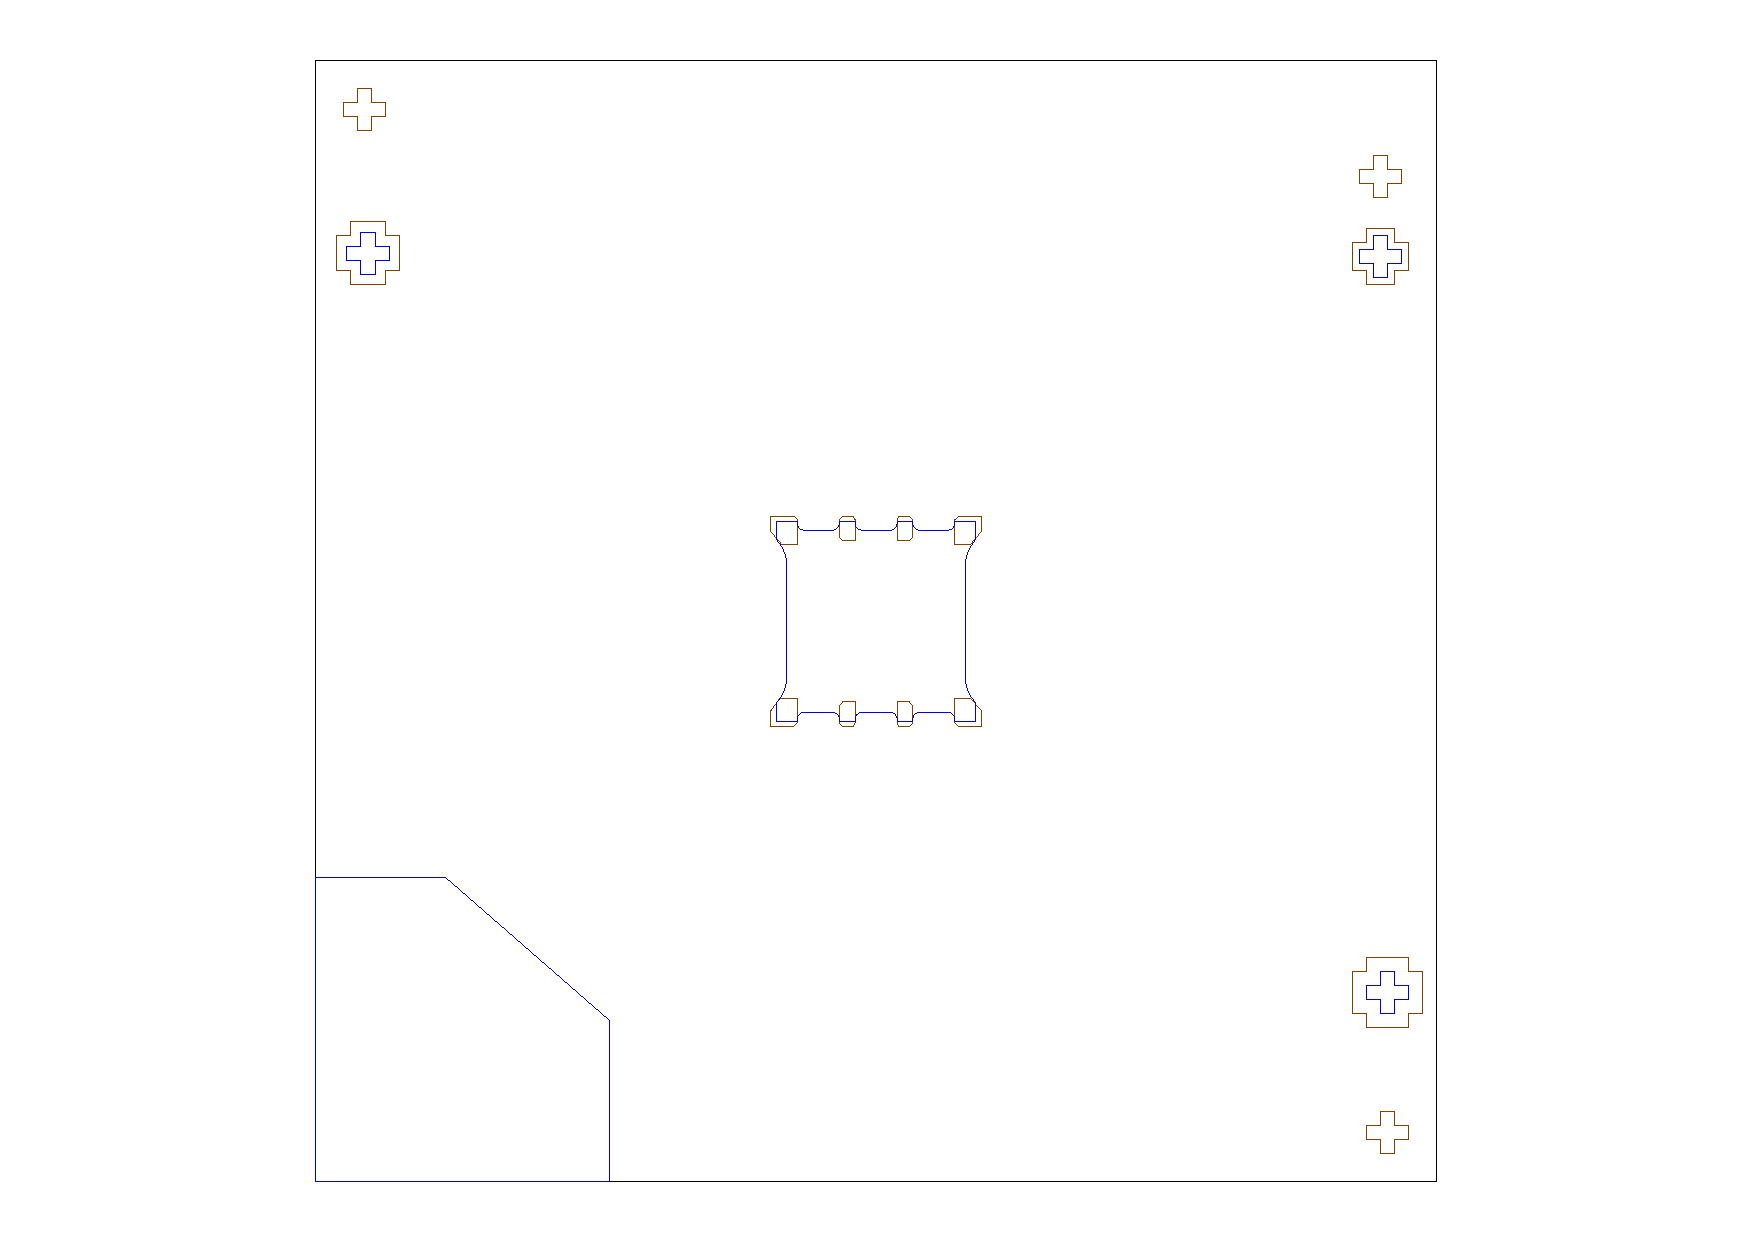
\includegraphics[scale=0.6]{fig/align1_1.pdf}
\caption{Picture of the geometry to expose. Can be used to write coordinates.} \label{align1}
\end{figure}

\newpage

\begin{figure} [h] \centering
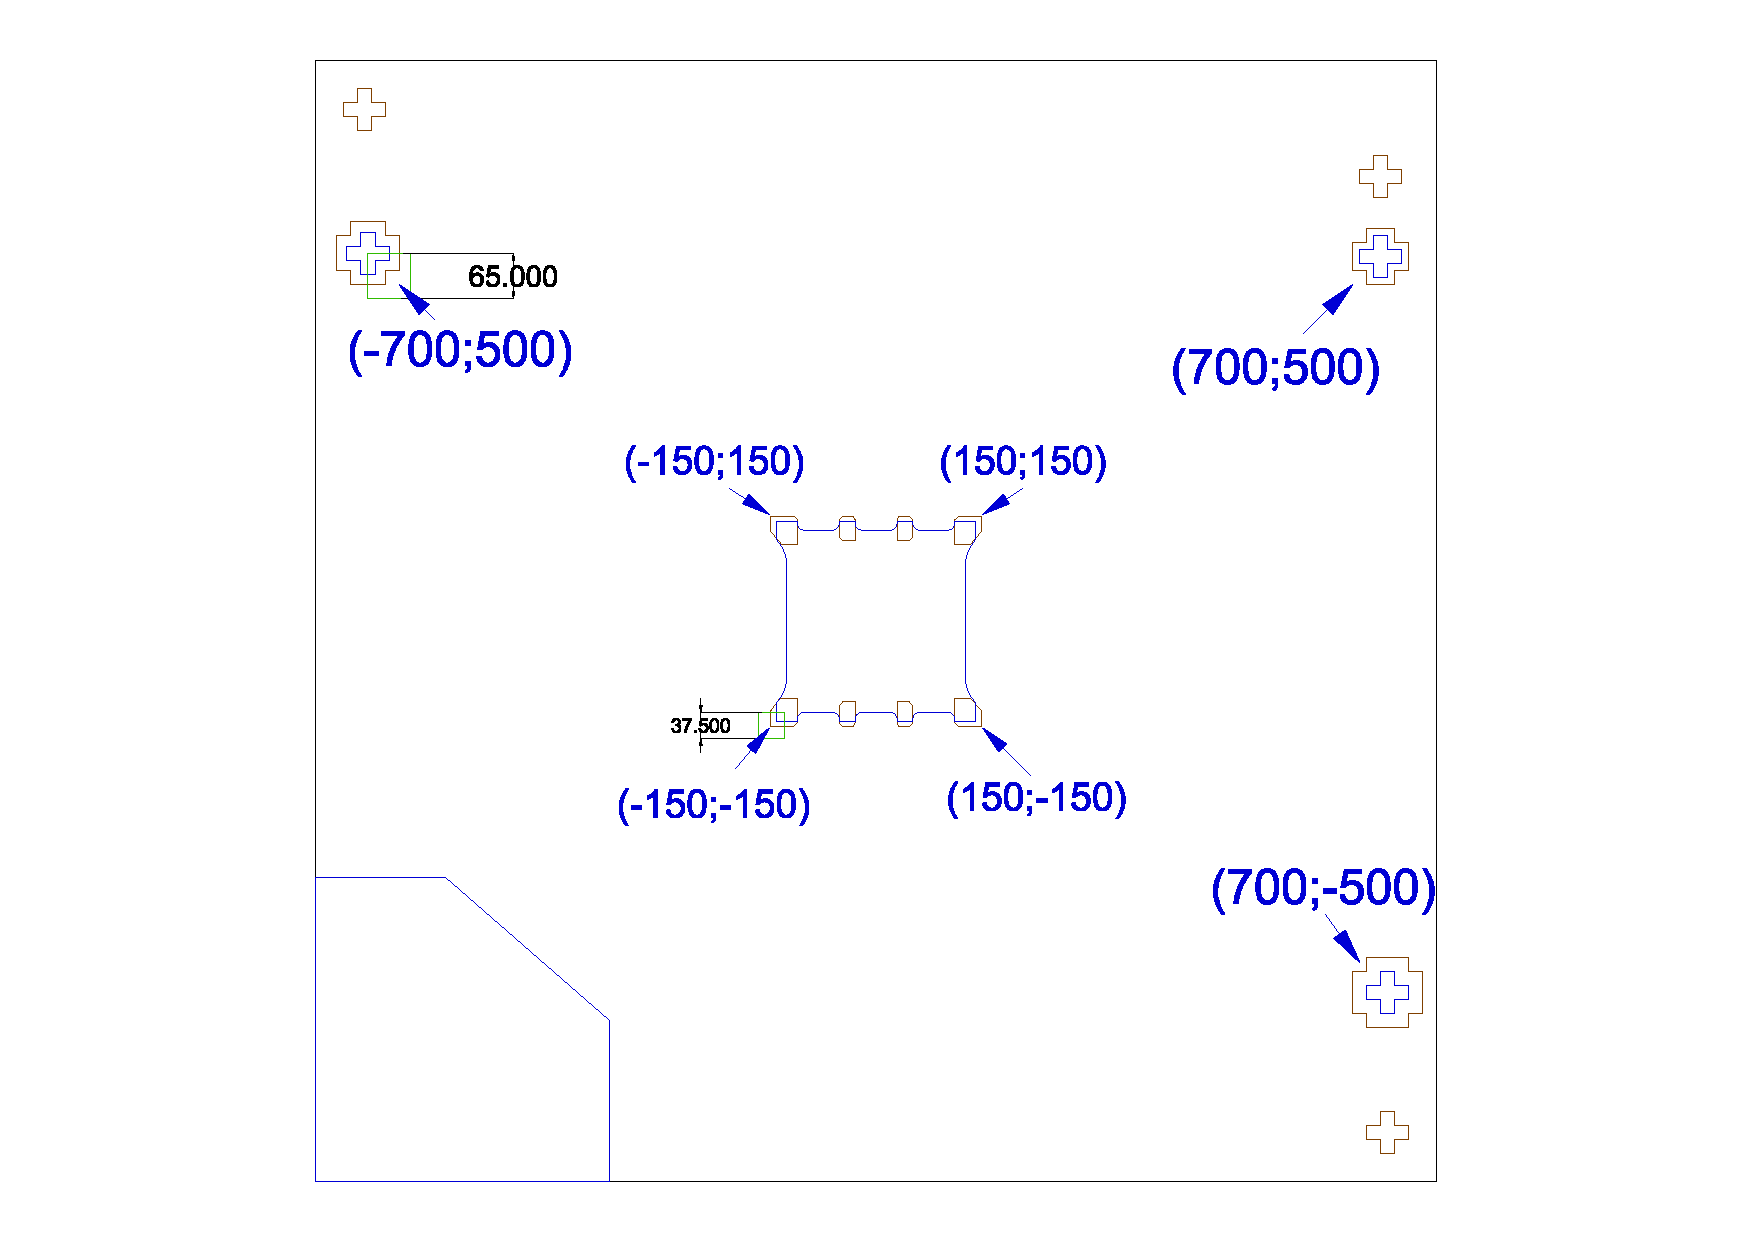
\includegraphics[scale=0.6]{fig/DD_Dots_V6_with_coord.pdf}
\caption{Marks coordinates for manual alignment. Coordinates won't change from one pattern to another, cause 
the marks are symmetric. Marks at the center are not to be used but in alignment problems (be careful about the exposing area).} \label{align1}
\end{figure}

\newpage

\begin{figure} [ht] \centering
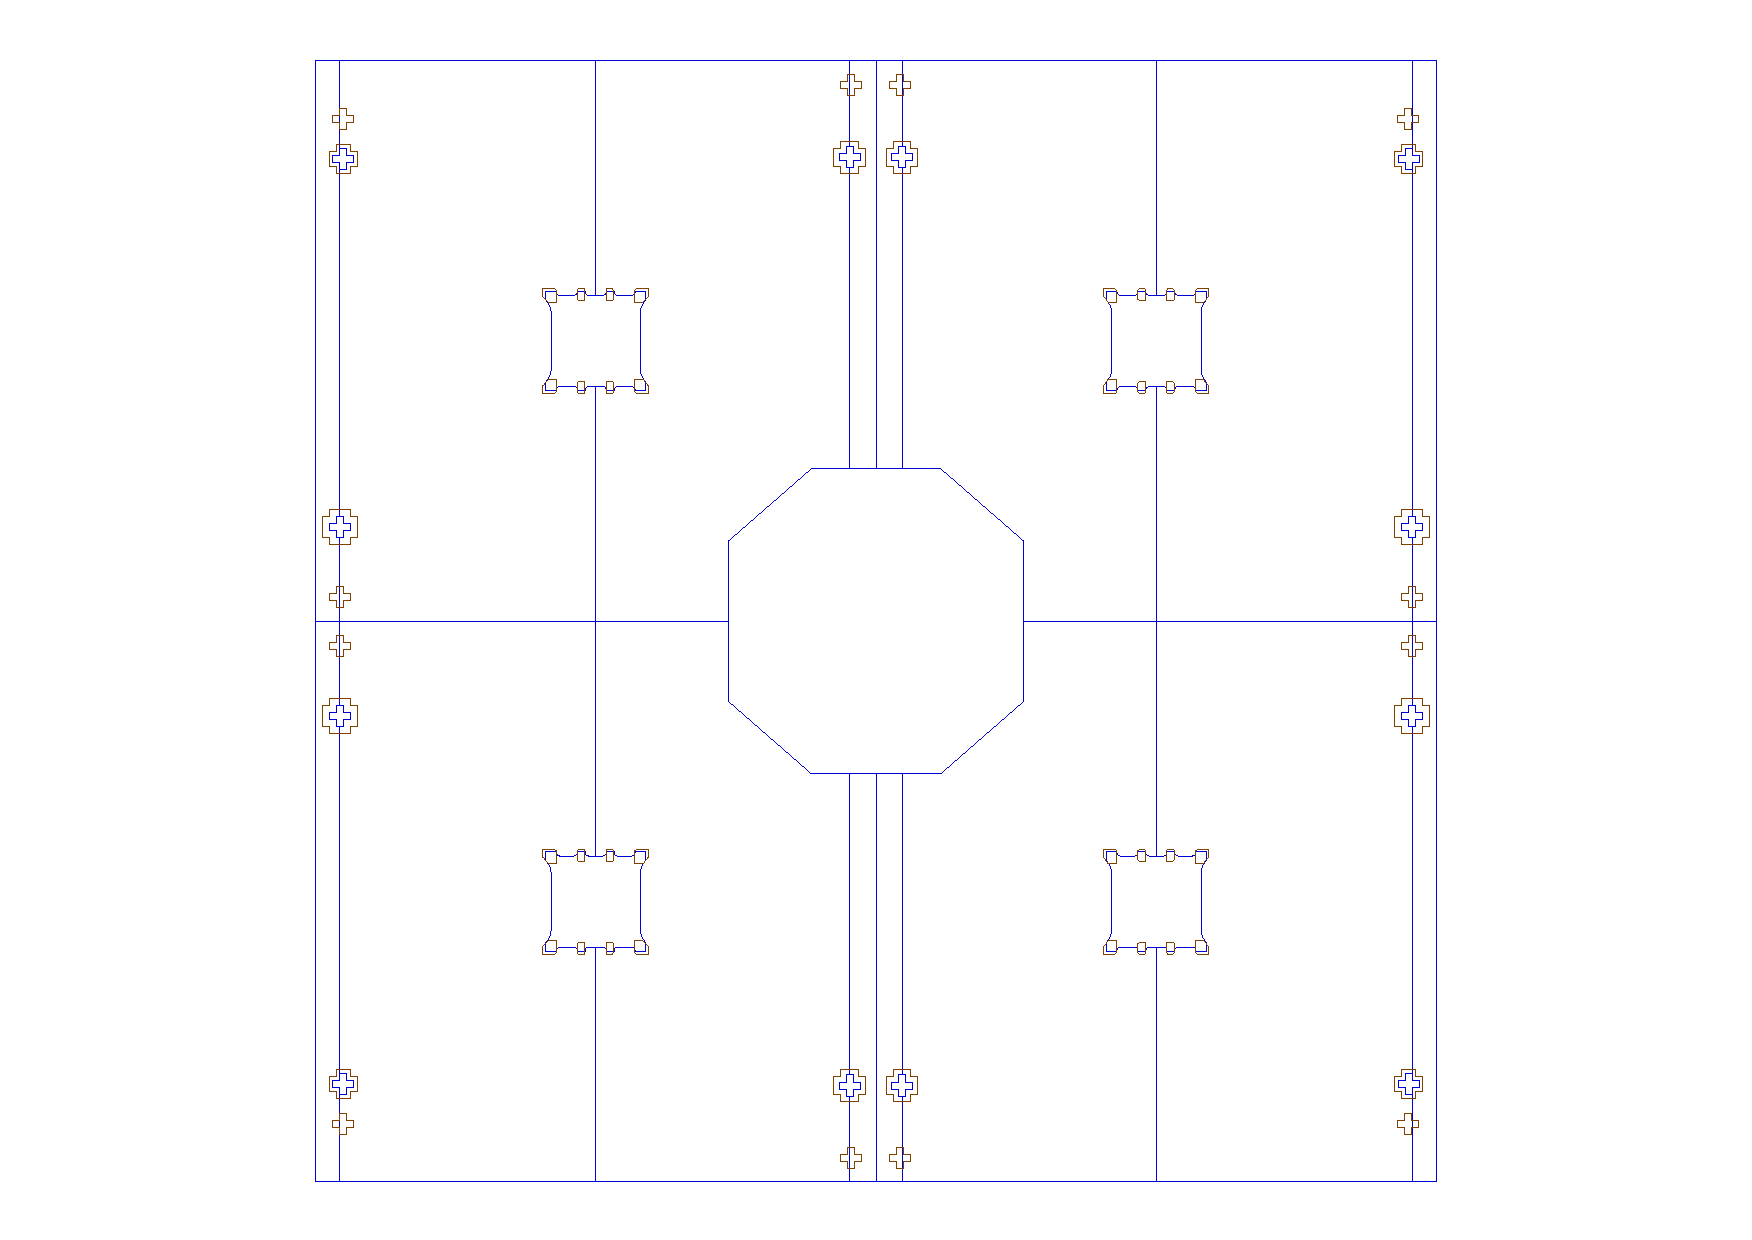
\includegraphics[scale=0.6]{fig/DD_Dots_V5_ebl_whole_mesa_ohmics.pdf}
\caption{Whole mask with mesa and ohmics} \label{align1}
\end{figure}

Size mesa : 840$\mu$m $\times$ 870$\mu$m. \\

UV coordinates of:\\

- Mark 1:~~~~~~~~~~~~~~~~~~~~~~~~~~~~~~~~~~~~~~~~~~~~~~~~ ; Mark 2: \\

- Mark 3:  \\

- center of mesa for gold balls: \\

- Ohmic corner 1:~~~~~~~~~~~~~~~~~~~~~~~~~~~~~~~~~~~~~~~~~; Ohmic corner 2:\\

- Ohmic corner 3:~~~~~~~~~~~~~~~~~~~~~~~~~~~~~~~~~~~~~~~~~; Ohmic corner 4:\\

\newpage

